In this section, we present our study results by answering our research questions. For each question, we discuss the motivation behind it, the approach to answering it and finally the results obtained. 
\\

\noindent\textbf{RQ1:} \textbf{How much do logs change over time and why do the changes occur?}
\\

\noindent\textbf{Motivation}

Research has shown that logs evolve along with the code~\cite{IanContextinformation}. When logs are changed, the log  processing tools which are dependent on them also have to get updated. This results in costly maintenance effort. To understand the cost, we have to understand how frequent changes to logs are. Hence, we explore the frequency of changes to logs in all our studied systems.\\

\noindent \textbf{Approach}

To find the frequency of log changes, we conduct a quantitative analysis on our studied systems. We use the tracked log data for each studied system as explained in Section~\ref{Methodology}. From each project, we select a random sample with 95\% confidence interval. We follow the same iterative process as in prior research~\cite{IanIcesm} to find how frequently logs change in our studied systems. \\

When logs are changed, they can be changed in several ways. To understand the different types of log changes we perform a manual analysis on the changed logs. We select a random sample from each project such that the sample achieves 95\% interval. After identifying all the types of log changes we automate the process using \textsl{Levenshtein ratio}~\cite{levenshteinratio}. Figure~\ref{fig:Flowchart2} highlights the process of categorizing the log changes. For example, 
consider the logs shown below. 

\hypobox {+ LOG.info(``starting HBase HsHA Thrift server on " + Integer.toString(listenPort)); }

\hypobox {- LOG.info(``starting HBase " + implType.simpleClassName() +`` server on " + Integer.toString(listenPort)); }


To identify the type of log change we first remove the logging method (i.e, LOG) and the log level (i.e, info) from the logs. We then compute the \textsl{Levenshtein ratio} between each term within the parentheses. In the above case we find that `+ Integer.toString(listenPort)' has \textsl{Levenshtein ratio} of 1, implying they are identical and the \textsl{Levenshtein ratio} between `starting HBase HsHA Thrift server on' and `starting HBase' is 0.56. This suggests there is some similarity between the two strings. Using this information we categorize logs into different types.

\begin{figure}[tb]
	\centering
	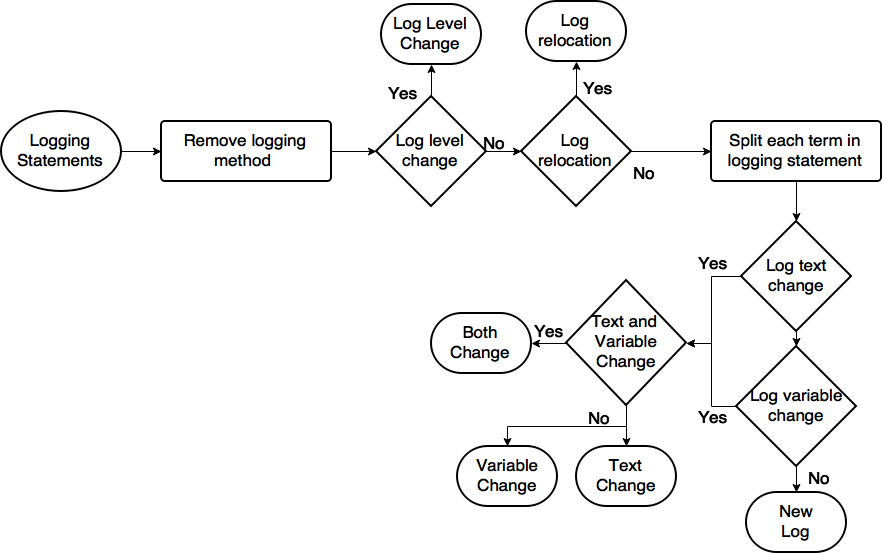
\includegraphics[width=0.75\linewidth]{Flowchart2v2}
	\caption{Flowchart to categorize the different types of log changes that occur}
	\label{fig:Flowchart2}
\end{figure}


\noindent \textbf{Results}

\textbf{We find that developers change 20-80\% of the logs across our studied systems as shown in Table~\ref{tba:logchangeDistribution}}. Based on frequency of changes, we categorize logs into 3 categories namely: a) Frequently Changed, b) Changed and c) Never Changed. If a log is changed more than three times it is categorized as `Frequently Changed'. If it is changed fewer than three times it is categorized under `changed' and if there is no changes made it is categorized under `Never Changed'. We see that `Never Changed' is majority only in Liferay and Camel but is lesser than `Changed' in ActiveMQ and CloudStack, as seen in Table~\ref{tba:logchangeDistribution}. This may be because Camel and Liferay rely less on logs as their middle-ware/application software, whereas ActiveMQ and CloudStack are service software.


\begin{table}[]
	\centering
	\caption{Distribution of log changes in different projects}
	\label{tba:logchangeDistribution}
	\begin{tabular}{l|lll}
	\cline{1-4}  	\multicolumn{1}{|c}{Projects}    & \multicolumn{1}{|c}{Never Changed (\%) }  &  \multicolumn{1}{|c}{Changed (\%) }	   &  \multicolumn{1}{|c}{Frequently Changed (\%) }\\ \cline{1-4}   

		Life Ray      & 78.67     & 19.66 & 1.66           \\
		
		Camel      & 55.43    & 37.32 & 7.25            \\
		ActiveMq   & 34.78     & 62.02 & 3.20           \\
		CloudStack & 19.68     & 68.61 & 11.71          \\ \cline{1-4}
	\end{tabular}
\end{table}

When developers change logs there can be many types of changes, i.e., changes to log context, verbosity levels or logged variables. From our manual analysis, we identify five types of log changes. Table~\ref{tba:logtype} shows their distributions. When there is overlapping of the different types of log changes, we categorize them as newly added log and track changes made to it.
\begin{enumerate}

\item { \textbf{Log relocation:} } The log is kept intact but moved to different location in the file because of context changes(code around the log is changed).

\item \textbf{Text change:} The text (i.e., static content) of log is changed. 

\item\textbf{Variable change:} One or more variables in the log are changed (added, deleted or modified).

\item \textbf{Change of log level:} The verbosity level of a log is changed.

\item  \textbf{Text and variable change:} Both text and variables in the logs are changed. This is generally done when developers provide more context information, i.e, text and add/modify the relevant variables in a log.

\end{enumerate}

Log relocation occurs more than other types of log changes. We find that in =all the studied systems log relocation occurs more than 40\%. As log relocations have no changes to the text or variables in logs, their impact on log processing tools is limited. Hence we exclude log relocation changes from our datasets. 


\begin{table}[t]
	\centering
	\caption{Distribution of log changes in different projects}
	\label{tba:logtype}
	\begin{tabular}{l|llll}
		\cline{1-5}  	\multicolumn{1}{|c}{Projects}    & \multicolumn{1}{|c}{ Life Ray }  &  \multicolumn{1}{|c}{ Cloud Stack}	   &  \multicolumn{1}{|c}{ Active-MQ }  & 
		 \multicolumn{1}{|c|}{ Camel } \\ \cline{1-5}   
		
		Log Relocation (\%)       & 73.5     & 78.85 &  63.27  & 49.72         \\
		
		Log Text Change (\%)      & 20.11    & 6.37 & 5.97    & 7.59       \\
		Log Variable Change (\%)   & 3.10     & 7.21 & 6.91 &  8.29     \\
		Change of Log Level (\%) & 0.87   & 1.15 & 1.76  &  3.79       \\ 
		Text and Variable Change (\%) & 2.33     & 6.39 & 22.0   &  30.59    \\ \cline{1-5}
	\end{tabular}
\end{table}

\hypobox { 45\% of the logs are changed atleast once in three of our studied systems. We find that over 50\% of these log changes are due to log relocation. The remaining changes are to the text (i.e., static content), variable and log level. This suggests that developers change logs extensively throughout the lifecyle of a software and developers might dedicate significant amount of time to update and maintain logs}
%	We find that about 3-11 \% of logs are changed frequently. This suggests that log processing tools which run on these systems need constant maintenance from developers

